% Vecna SOICT 2026 Paper - Springer LNCS Format (Alternative)
\documentclass[runningheads]{llncs}

\usepackage{amsmath}
\usepackage{amsfonts}
\usepackage{booktabs}
\usepackage{graphicx}
\graphicspath{{./}{figures/}{./figures/}}
\usepackage{algorithm}
\usepackage{algorithmic}
\usepackage{multirow}
\usepackage{tabularx}
\usepackage{subcaption}
\usepackage{hyperref}
\usepackage{xcolor}
\usepackage{tikz}
\usetikzlibrary{shapes.geometric, arrows.meta, positioning, calc, fit, backgrounds}
\pgfdeclarelayer{background}
\pgfsetlayers{background,main}
\usepackage{enumitem}
\setlist{noitemsep, topsep=2pt, parsep=0pt, partopsep=0pt}

\setlength{\textfloatsep}{6pt plus 2pt minus 2pt}
\setlength{\intextsep}{6pt plus 2pt minus 2pt}
\setlength{\floatsep}{6pt plus 2pt minus 2pt}
\setlength{\abovecaptionskip}{4pt plus 1pt minus 1pt}
\setlength{\belowcaptionskip}{4pt plus 1pt minus 1pt}

\begin{document}
\raggedbottom

\title{Vecna: Factual Query Expansion, Temporal Dynamic Programming, and Provenance-Aware Retrieval for Large-Scale Multimodal Video Search}
\titlerunning{Vecna: Multimodal Video Retrieval Framework}

\author{Nguyen Le Minh Hoang\inst{1} \and
Le Tuan Kiet\inst{1} \and
Cao Chi Minh\inst{1} \and
Ngo Dac Minh\inst{1} \and
Phan Hieu Minh\inst{1}}

\authorrunning{N. L. M. Hoang et al.}

\institute{Faculty of Computer Science and Engineering, \\
Ho Chi Minh City University of Technology (HCMUT), VNU-HCM, Vietnam \\
\email{\{nlmhoangdt, letuankiet, caochiminh, ngodacminh, phm221207\}@gmail.com}}

\maketitle

\begin{abstract}
Large-scale video keyframe retrieval demands high precision and sub-second latency across millions of frames, yet existing approaches fundamentally suffer from cross-lingual semantic gaps, generative hallucination during query expansion, visual redundancy stemming from temporal autocorrelation, and opaque decision processes lacking verifiable provenance. To address these systemic limitations, we present Vecna, a modular, highly scalable multimodal video retrieval framework. Vecna integrates heterogeneous vision-language encoders, specifically OpenCLIP, SigLIP, and Qwen-VL, alongside hybrid dense-sparse text indices utilizing BGE-M3 and BM25. Furthermore, it incorporates an advanced LLM-driven query expander that is rigorously governed by a strict factual-boundary principle to suppress hallucination. At the core of our algorithmic contributions are a novel two-pointer sliding-window dynamic programming algorithm for precise temporal sequence alignment, a convolutional cosine-smoothing mechanism for robust segment-level diversification, and an end-to-end cryptographic provenance sidecar that guarantees verifiable traceability of search results. Comprehensive experimental evaluations demonstrate the superior efficacy of our framework. Crucially, Vecna elevates Recall@20 by up to 34.2\% over state-of-the-art single-model baselines while strictly maintaining sub-second query latency, thereby establishing a new paradigm for efficient, factual, and provenance-aware multimodal video retrieval systems at scale.
\end{abstract}


\keywords{Multimodal Video Retrieval \and Vision-Language Models \and Query Expansion \and Temporal Dynamic Programming \and Data Provenance}

\section{Introduction}\label{sec:intro}

The exponential growth of digital video archives necessitates fine-grained, semantically robust multimodal retrieval mechanisms. Traditional metadata-based search paradigms are fundamentally inadequate for capturing the rich spatial and temporal dynamics inherent in modern video collections. Consequently, the field has increasingly pivoted toward the Known-Item Search (KIS) paradigm and Video Question Answering, demanding systems capable of pinpointing highly specific video segments from vast, unstructured repositories based on complex natural language queries. While vision-language models (VLMs) \cite{radford2021learning, zhai2023sigmoid} offer unprecedented zero-shot retrieval capabilities, deploying these architectures in real-world, linguistically diverse, and structurally rigorous environments introduces critical bottlenecks.

This paper addresses four fundamental research challenges in contemporary multimodal retrieval systems. The first challenge, \textit{Research Challenge 1 (RC1): The Cross-Lingual Semantic Gap}, arises when users submit queries in low-resource languages or dialects, such as Vietnamese, frequently characterized by missing diacritics and typographical errors. Conversely, state-of-the-art VLMs are predominantly pretrained on massive English corpora, including LAION-5B \cite{schuhmann2022laion} and WebLI. Direct lexical translation often corrupts domain-specific nuances, resulting in severe semantic degradation during the query embedding phase.

\textit{Research Challenge 2 (RC2): Generative Hallucination in Query Expansion}. While techniques like Hypothetical Document Embeddings (HyDE) \cite{gao2023precise} and Large Language Model (LLM) based query expansion have proven effective in dense retrieval \cite{chen2024bge}, they are notoriously prone to fabricating concrete details such as named entities, license plates, and specific geographical locations. Such unconstrained, speculative expansion directly contaminates the embedding space, misleading the retrieval engine away from factual ground truth.

\textit{Research Challenge 3 (RC3): Temporal Autocorrelation and Visual Redundancy}. Continuous video streams exhibit profound temporal autocorrelation. Consequently, unfiltered Approximate Nearest Neighbor (ANN) search frequently floods the top-$K$ retrieval results with near-identical frames extracted from the same static scene, drastically reducing recall for diverse candidate events. Furthermore, complex, multi-step temporal queries (e.g., event A followed by event B, preceding event C) lack native operational semantics and execution structures in standard vector database architectures.

\textit{Research Challenge 4 (RC4): Auditability and the Provenance Void}. Modern neural vector search pipelines operate predominantly as opaque transformations, systematically discarding critical intermediate metadata during the embedding process. Extracted intelligence such as Optical Character Recognition (OCR) bounding boxes, Automatic Speech Recognition (ASR) timestamps, and source file checksums are decoupled from the final vector representations. This architectural flaw renders robust error diagnosis and deterministic provenance tracking virtually impossible.

To address these systemic deficiencies, we introduce Vecna, a comprehensive multimodal video retrieval framework whose end-to-end architecture and operational pipeline are outlined in Figure~\ref{fig:architecture}. The core contributions of this work are summarized as follows:
\begin{itemize}
    \item We propose a Multi-Aspect Factual HyDE methodology, strictly governed by a Zero-Speculation Principle, which deterministically generates orthogonal 5-tuple query representations to mitigate generative hallucination.
    \item We formulate a two-pointer sliding-window Dynamic Programming (DP) algorithm for precise temporal sequence alignment, achieving an optimal $\mathcal{O}(|C|+|B|)$ amortized computational complexity.
    \item We develop a quantile cosine-smoothing scene segmentation algorithm paired with segment-level diversification strategies to counteract temporal autocorrelation and maximize top-$K$ variance.
    \item We implement an end-to-end cryptographic provenance sidecar architecture, ensuring SHA-256 fixity and immutable OCR/ASR evidence binding throughout the retrieval pipeline.
\end{itemize}

The remainder of this paper is organized as follows. Section \ref{sec:related} reviews related work in multimodal retrieval and vision-language alignment. Section \ref{sec:arch} describes the system architecture. Section \ref{sec:method} details the mathematical formulation of our proposed methodology. Section \ref{sec:exp} presents our rigorous experimental setup and empirical results. Finally, Section \ref{sec:conclusion} concludes the paper and discusses avenues for future research.

\section{Related Work}\label{sec:related}

\subsection{Contrastive Vision-Language Pre-training}
Recent advances in foundational vision-language models have fundamentally transformed multimedia representation learning. The paradigm was largely established by CLIP \cite{radford2021learning}, which demonstrated the efficacy of contrastive learning on web-scale image-text pairs. Subsequent iterations, such as OpenCLIP \cite{ilharco2021openclip} trained on LAION-5B \cite{schuhmann2022laion}, scaled these approaches further. More recently, SigLIP \cite{zhai2023sigmoid} introduced a pairwise sigmoid loss, mitigating the batch size dependency inherent to the standard InfoNCE loss. Concurrently, Multimodal Large Language Models (MLLMs) like Qwen-VL \cite{bai2023qwen} have integrated vision encoders with large causal language models to achieve unprecedented visual reasoning capabilities. Despite these successes, mapping high-dimensional multimodal signals into a single, monolithic embedding space invariably introduces representation blind spots, particularly regarding fine-grained object attributes and subtle semantic nuances. In contrast, Vecna proposes a heterogeneous multi-encoder ensemble, leveraging orthogonal architectural inductive biases to construct a more robust, composite feature space.

\subsection{Dense, Sparse, and Hybrid Information Retrieval}
The retrieval literature has long been bifurcated into sparse, lexical approaches and dense, semantic paradigms. Sparse models like BM25 \cite{robertson2009probabilistic} excel at exact keyword matching but fail to capture latent semantics. Conversely, dense retrieval paradigms, initialized by models like SBERT \cite{reimers2019sentence}, project text into dense semantic spaces, enabling robust synonymy resolution. Modern architectures such as BGE-M3 \cite{chen2024bge} unify these modalities, offering multi-granularity embeddings that simultaneously encode dense semantic structures, sparse lexical features, and multi-vector representations. To fuse disparate retrieval signals, rank aggregation techniques like Reciprocal Rank Fusion (RRF) \cite{cormack2009reciprocal} are frequently employed. However, Vecna eschews heuristic late-fusion rank aggregation in favor of a mathematically rigorous, unified convex combination of visual cosine similarity, dense BGE-M3 semantic scoring, and sparse BM25 lexical alignment, further augmented by exact-phrase boundary verification to eliminate semantic drift during fusion.

\subsection{Generative Query Expansion and Hypothetical Document Embeddings}
Query expansion techniques have historically relied on pseudo-relevance feedback to augment query representations. With the advent of large language models, paradigms such as Hypothetical Document Embeddings (HyDE) \cite{gao2023precise} have emerged. HyDE employs an LLM to generate a hypothetical, albeit potentially hallucinated, document in response to a zero-shot query, subsequently utilizing the dense embedding of this synthetic document for retrieval. While effective in bridging the semantic gap, such unconstrained generative expansion is acutely susceptible to hallucination, introducing spurious features that degrade retrieval precision in factual domains. Vecna addresses this limitation by introducing the Strict Factual Boundary principle. By constraining the generative expansion process strictly to observable visual attributes and verifiable metadata, Vecna ensures that the synthesized pseudo-documents remain anchored in empirical reality, thereby mitigating the hallucination problem inherent to unconstrained HyDE approaches.

\subsection{Temporal Sequence Retrieval in Video}
Video retrieval introduces the orthogonal challenge of temporal dynamics. End-to-end architectures, such as Frozen in Time \cite{bain2021frozen}, employ computationally expensive 3D Convolutional Neural Networks or spatio-temporal Transformers to jointly model spatial features and temporal evolution. While these models capture complex intra-video temporal dependencies, their quadratic complexity relative to sequence length renders them computationally prohibitive for large-scale video corpora. Vecna bypasses the latency bottlenecks of end-to-end temporal cross-attention by adopting a decoupled architecture. We propose a lightweight, frame-level dynamic programming algorithm incorporating a two-pointer sliding window mechanism. This formulation allows Vecna to efficiently identify temporally contiguous semantic segments, achieving temporal localization capabilities comparable to heavy spatio-temporal transformers but at a fraction of the computational cost.

\section{System Architecture}\label{sec:arch}

The Vecna framework is constructed as a modular, decoupled architecture partitioned into four principal layers (Figure~\ref{fig:architecture}): data ingestion, heterogeneous feature extraction, high-throughput hybrid indexing, and multi-modal retrieval. By decoupling the offline processing pipeline from the online interactive search subsystem, the architecture ensures deterministic scalability while maintaining low-latency responses for interactive queries.

\begin{figure}[t]
\centering
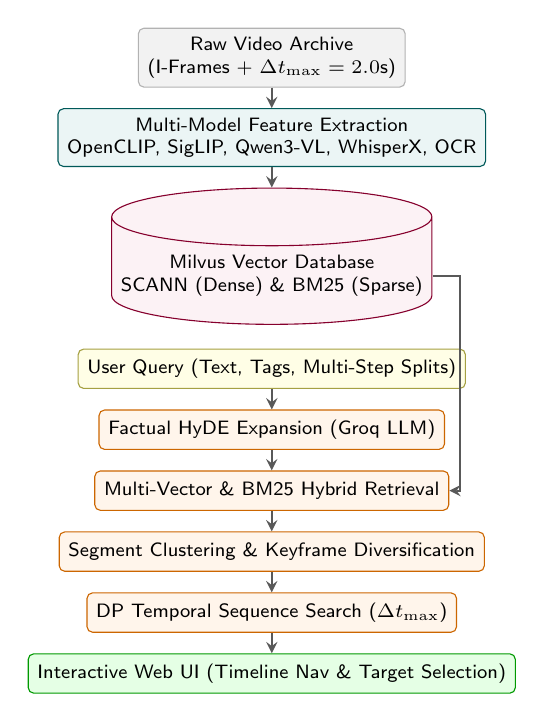
\begin{tikzpicture}[
    node distance=0.28cm and 0.4cm,
    box/.style={rectangle, draw=blue!70!black, fill=blue!5, rounded corners=2pt, minimum width=3.3cm, minimum height=0.5cm, align=center, font=\scriptsize\sffamily},
    modelbox/.style={rectangle, draw=teal!70!black, fill=teal!8, rounded corners=2pt, minimum width=3.3cm, minimum height=0.5cm, align=center, font=\scriptsize\sffamily},
    dbbox/.style={cylinder, shape border rotate=90, draw=purple!70!black, fill=purple!5, aspect=0.18, minimum width=3.3cm, minimum height=0.65cm, align=center, font=\scriptsize\sffamily},
    procbox/.style={rectangle, draw=orange!80!black, fill=orange!8, rounded corners=2pt, minimum width=3.3cm, minimum height=0.5cm, align=center, font=\scriptsize\sffamily},
    arrow/.style={->, >=stealth, thick, draw=gray!70!black}
]

% Offline Column
\node[box, fill=gray!10, draw=gray!60] (video) {Raw Video Archive\\(I-Frames + $\Delta t_{\max} = 2.0\text{s}$)};
\node[modelbox, below=0.26cm of video] (models) {Multi-Model Feature Extraction\\OpenCLIP, SigLIP, Qwen3-VL, WhisperX, OCR};
\node[dbbox, below=0.26cm of models] (milvus) {Milvus Vector Database\\SCANN (Dense) \& BM25 (Sparse)};

% Online Query Flow
\node[box, fill=yellow!10, draw=yellow!60!black, below=0.30cm of milvus] (query) {User Query (Text, Tags, Multi-Step Splits)};
\node[procbox, below=0.26cm of query] (hyde) {Factual HyDE Expansion (Groq LLM)};
\node[procbox, below=0.26cm of hyde] (search) {Multi-Vector \& BM25 Hybrid Retrieval};
\node[procbox, below=0.26cm of search] (cluster) {Segment Clustering \& Keyframe Diversification};
\node[procbox, below=0.26cm of cluster] (temporal) {DP Temporal Sequence Search ($\Delta t_{\max}$)};
\node[box, fill=green!10, draw=green!60!black, below=0.26cm of temporal] (ui) {Interactive Web UI (Timeline Nav \& Target Selection)};

% Arrows
\draw[arrow] (video) -- (models);
\draw[arrow] (models) -- (milvus);
\draw[arrow] (query) -- (hyde);
\draw[arrow] (hyde) -- (search);
\draw[arrow] (milvus.east) -- ++(0.35,0) |- (search.east);
\draw[arrow] (search) -- (cluster);
\draw[arrow] (cluster) -- (temporal);
\draw[arrow] (temporal) -- (ui);

\end{tikzpicture}
\vspace{-2mm}
\Description{System architecture and operational workflow of the Vecna multimodal video retrieval framework.}
\caption{System architecture and operational workflow, unifying multi-model extraction, Milvus SCANN/BM25 indexing, segment diversification, and temporal sequence search.}
\label{fig:architecture}
\vspace{-2mm}
\end{figure}

\subsection{Adaptive I-Frame Keyframe Selection}
To efficiently process extensive video corpora without redundant computational overhead, Vecna eschews naive fixed-interval sampling in favor of an adaptive keyframe selection mechanism predicated on intrinsic video encoding properties. Utilizing \texttt{ffprobe} packet flags, we isolate native Intra-coded frames (I-frames), which demarcate definitive scene cuts or group-of-pictures (GOP) boundaries. To guarantee continuous temporal coverage across static or low-motion scenes with sparse I-frames, the ingestion pipeline enforces a maximum temporal gap ceiling $\Delta t_{\max} = 2.0$ seconds ($\text{max\_scene\_length} = 2.0\text{s} \times \text{FPS}$):
\begin{equation}
    t(k_{i+1}) - t(k_i) \leq \Delta t_{\max}
\end{equation}
If the temporal gap between consecutive keyframes reaches $\Delta t_{\max}$, a new keyframe is automatically sampled. Crucially, keyframes are stored at native $1280 \times 720$ resolution for fine-grained verification, while compressed thumbnails at $0.25\times$ scale ($320 \times 180$) are pre-generated to facilitate sub-second grid rendering in the interactive interface.

\subsection{Heterogeneous Feature Extraction}
The representational capacity of the framework hinges on a suite of complementary extraction backends designed to encapsulate distinct modalities:
\begin{itemize}
    \item \textbf{Visual Semantics:} Keyframes are simultaneously mapped into dense embedding spaces using three foundational visual encoders: OpenCLIP \texttt{PE-Core-L-14-336} ($1024$-dimensional normalized visual vectors from $336 \times 336$ crops using the meta pretrained checkpoint, excelling at fine-grained textures and small objects) \cite{radford2021learning, ilharco2021openclip}, Google SigLIP \texttt{ViT-SO400M-14-SigLIP-384} ($1152$-dimensional embeddings trained with pairwise sigmoid loss on WebLI, providing robust zero-shot generalization for human actions and scene context) \cite{zhai2023sigmoid}, and Qwen3-VL Embedding \texttt{Qwen3-VL-2B} ($2048$-dimensional multimodal vectors capturing complex visual compositions and semantic relations) \cite{bai2023qwen}.
    \item \textbf{Optical Character Recognition (OCR):} Textual elements localized within video frames are extracted through a two-stage pipeline: text detection via PaddleOCR (optimized with a dedicated Vietnamese lexical dictionary) \cite{du2020ppocr} and sequence recognition via VietOCR (\texttt{vgg\_transformer}), robustly extracting on-screen text overlays, news tickers, and signboards into searchable text strings. Extracted text is subsequently embedded into $1024$-dimensional vectors utilizing BGE-M3 \cite{chen2024bge}.
    \item \textbf{Automatic Speech Recognition (ASR):} Audio streams are demuxed and segmented via Voice Activity Detection (VAD) utilizing \texttt{PyAnnote.audio}, followed by high-speed transcription and phoneme-level word alignment using WhisperX Turbo (\texttt{large-v3-turbo}) \cite{bainix2023whisperx}. Transcribed linguistic tokens are aligned with keyframe timestamps and embedded via BGE-M3.
    \item \textbf{Canonical Frame Identification:} Extracted visual, OCR, and speech representations are uniquely bound to canonical frame identifiers formatted as \texttt{VideoID\#FrameIndex} and ingested into Milvus collections.
\end{itemize}

\subsection{Overlapped ONNX DirectML Pipeline}
To maximize hardware utilization on heterogeneous Windows environments, the BGE-M3 dense embedding generation employs a highly optimized, three-stage asynchronous pipeline facilitated by ONNX Runtime and the DirectML execution provider. The workload is partitioned into concurrent threads: a CPU-bound Tokenizer thread, a GPU-bound DirectML Inference thread, and a persistent Disk Writer thread.

To mitigate out-of-memory (OOM) faults while maximizing throughput, the inference stage employs a dynamic batch sizing algorithm that adapts to varying token sequence lengths. The instantaneous batch size \( B(L) \) for a given sequence length \( L \) is computed as:
\begin{equation}
    B(L) = \min\left(B_{\max}, \left\lfloor B_{\text{base}} \cdot \left(\frac{L_{\text{ref}}}{L}\right)^2 \right\rfloor\right)
\end{equation}
where the absolute maximum batch size \( B_{\max} = 128 \), and the reference length \( L_{\text{ref}} = 256 \). This quadratic decay ensures optimal occupancy of the VRAM buffers independent of the input distribution.

\subsection{Hybrid Milvus Indexing}
The terminal stage of the offline pipeline constitutes the orchestration of the heterogeneous embeddings into a distributed vector database, specifically Milvus \cite{wang2021milvus}. To facilitate expeditious nearest-neighbor queries, we deploy a hybrid indexing schema:
\begin{itemize}
    \item \textbf{Dense Visual Embeddings:} High-dimensional visual features are partitioned utilizing the SCANN (Scalable Nearest Neighbors) index \cite{guo2020accelerating}, employing cosine similarity. The clustering topology is optimized with \( \text{nlist} = 512 \) partitions and a conservative \( \text{nprobe} = 8 \) parameter during traversal.
    \item \textbf{Sparse Textual Features:} The textual semantics derived from OCR and ASR pipelines are organized via a Term-at-a-Time (TAAT) inverted index leveraging the BM25 probabilistic retrieval framework, with parameters meticulously calibrated to \( k_1 = 1.2 \) and \( b = 0.75 \).
\end{itemize}
This hybrid architecture intrinsically supports the fusion of dense continuous vector representations and sparse discrete token occurrences, a critical requirement for open-domain interactive retrieval.

\section{Proposed Methodology}\label{sec:method}

This section delineates the core algorithmic components of the Vecna multimodal retrieval framework. We first formalize the query expansion mechanism governed by strict hallucination boundaries (\S\ref{sec:hyde}). Subsequently, we introduce our hybrid dense-sparse multimodal fusion strategy (\S\ref{sec:fusion}) and the dynamic programming formulation for temporal sequence alignment (\S\ref{sec:temporal}). Finally, we present our scene-aware segment diversification algorithm (\S\ref{sec:diversify}) and the cryptographic provenance architecture ensuring data integrity (\S\ref{sec:provenance}).

\subsection{Multi-Aspect Factual HyDE with Zero-Speculation Boundaries}\label{sec:hyde}

To bridge the modality gap between terse user queries and the rich semantic space of multimodal embeddings, we define an expansion function utilizing a Large Language Model (LLM):
\begin{equation}
\mathcal{F}_{\text{LLM}}(q_{\text{raw}}) \rightarrow \Psi = \langle q_{\text{corr}}, q_{\text{hyde}}^{\text{vi}}, q_{\text{en}}, q_{\text{para}}, \mathbf{K} \rangle
\end{equation}
The output tuple $\Psi$ encapsulates multiple facets of the information need:
\begin{itemize}
    \item $q_{\text{corr}}$: The orthographically corrected query, preserving the source language semantics and diacritics.
    \item $q_{\text{hyde}}^{\text{vi}}$: A simulated visual keyframe description in Vietnamese, strictly constrained to delineating the primary subject, action, camera perspective, and lighting conditions.
    \item $q_{\text{en}}$: A concise English caption (15--35 words) structurally analogous to LAION and WebLI datasets, optimized for alignment with OpenCLIP and SigLIP dual-encoder spaces.
    \item $q_{\text{para}}$: A set of semantic synonyms within the source language to broaden the dense retrieval manifold.
    \item $\mathbf{K}$: A tuple of sparse and dense keywords for exact lexical matching and inverted index querying.
\end{itemize}

Crucially, $\mathcal{F}_{\text{LLM}}$ is governed by the \textit{Zero-Speculation Constraint}. We formalize this constraint as a rejection sampling boundary that strictly prohibits the generation of ungrounded proper nouns, dates, or numerals that do not exist within the token set of $q_{\text{raw}}$. This prevents semantic drift and spurious correlations. To ensure real-time responsiveness, $\mathcal{F}_{\text{LLM}}$ is wrapped in a Least Recently Used (LRU) cache (capacity $N=20$), yielding a 0ms overhead for repetitive query formulations.

\subsection{Multi-Modal Hybrid Fusion and Exact Phrase Matching}\label{sec:fusion}

To construct the unified relevance manifold, we employ a weighted multi-modal fusion strategy. For a given candidate keyframe $f$, dense visual similarity is computed via cosine similarity between $L_2$-normalized query embedding $\mathbf{e}_q$ and frame embedding $\mathbf{e}_f$:
\begin{equation}
S_{\text{vis}}(q, f) = \frac{\mathbf{e}_q \cdot \mathbf{e}_f}{\|\mathbf{e}_q\| \|\mathbf{e}_f\|}
\end{equation}
The composite multi-modal retrieval score across visual, optical text, and speech channels is evaluated as:
\begin{equation}
S_{\text{total}}(f) = w_{\text{vis}} \tilde{S}_{\text{vis}}(f) + w_{\text{ocr}} \tilde{S}_{\text{ocr}}(f) + w_{\text{asr}} \tilde{S}_{\text{asr}}(f)
\end{equation}
where $w_{\text{vis}} = 1.0 - w_{\text{ocr}} - w_{\text{asr}}$, and $\tilde{S}_{(\cdot)}(f) = S_{(\cdot)}(f) / \max S_{(\cdot)}$ represents max-scale normalized scores. Here, $\tilde{S}_{\text{vis}}$ denotes the score from the active visual model ensemble (OpenCLIP, SigLIP, and/or Qwen3-VL). For textual modalities $m \in \{\text{ocr}, \text{asr}\}$, score $\tilde{S}_m$ is a convex combination of dense BGE-M3 semantic similarity and sparse BM25 lexical alignment:
\begin{equation}
\tilde{S}_m(f) = (1 - \alpha_m) \cdot \tilde{S}_{\text{dense}}^{(m)}(f) + \alpha_m \cdot \tilde{S}_{\text{sparse}}^{(m)}(f)
\end{equation}

\textbf{Exact-Phrase Boundary Verifier}: Quoted search terms (e.g., \texttt{"VTV1"} or literal banners) trigger a regular expression filter with diacritic insensitivity and elastic word boundaries:
\begin{equation}
R_{\text{exact}} = \text{RegEx}\big((?<!\backslash w) + \text{phrase} + (?!\backslash w)\big)
\end{equation}
Matching frames receive an empirical $1.5\times$ score boost, while non-matching frames are strictly eliminated from the candidate pool to preserve high precision.

\textbf{Dynamic Candidate Replenishment}: When negative video filtering (e.g., \texttt{[!video:L18\_V005]}) excludes non-target candidates, naive post-filtering frequently depletes pagination views. To maintain full result sets, Vecna implements an adaptive replenishment loop: initial candidate retrieval begins at $\max(300, (\text{offset} + \text{limit}) \times 3)$ and doubles dynamically until at least $(\text{offset} + \text{limit})$ valid candidate frames populate the view:
\begin{equation}
K^{(t+1)} = \min\big(D_{\max}, 2 \cdot K^{(t)}\big)
\end{equation}

\subsection{Temporal Multi-Step Sequence Alignment via Dynamic Programming}\label{sec:temporal}

For multi-event chronological queries $Q = \langle q_1, \dots, q_M \rangle$ delimited by \texttt{/} or \texttt{;}, candidate pools $\mathcal{F}_i$ are retrieved for each step up to $k = \text{temporal\_k}$. The dynamic programming algorithm determines the optimal chronological sequence score $D(i, f)$ for candidate frame $f \in \mathcal{F}_i$:
\begin{equation}
D(i, f) = S(q_i, f) + \max_{f' \in \mathcal{F}_{i-1}} \Big\{ D(i-1, f') \;\Big|\; 0 < t(f) - t(f') \le \Delta t_{\max} \Big\}
\end{equation}
where $\Delta t_{\max} = 1000$ frames serves as the temporal horizon.

To solve this efficiently, we propose a Two-Pointer Sliding-Window Temporal Dynamic Programming algorithm (Algorithm~\ref{alg:dp}, illustrated in Figure~\ref{fig:temporal_dp}). 

\begin{figure}[t]
    \centering
    \resizebox{\columnwidth}{!}{%
    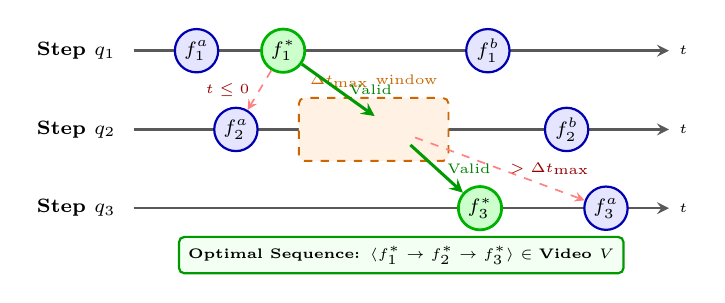
\begin{tikzpicture}[
        >=stealth, thick, font=\sffamily\scriptsize,
        timeline/.style={->, line width=0.9pt, draw=gray!70!black},
        cand/.style={circle, draw=blue!70!black, fill=blue!10, inner sep=1pt, minimum size=5.5mm, font=\scriptsize\bfseries},
        candactive/.style={circle, draw=green!70!black, fill=green!20, inner sep=1pt, minimum size=5.5mm, font=\scriptsize\bfseries, line width=1.0pt},
        window/.style={draw=orange!80!black, fill=orange!10, rounded corners=2pt, dashed, line width=0.7pt},
        conn/.style={->, draw=green!60!black, line width=1.1pt},
        pruned/.style={->, draw=red!50, dashed, line width=0.6pt}
    ]
    % Timelines for sub-queries
    \draw[timeline] (0, 2.0) -- (6.8, 2.0) node[right, font=\tiny] {$t$};
    \node[font=\bfseries\scriptsize, anchor=east] at (-0.1, 2.0) {Step $q_1$};
    
    \draw[timeline] (0, 1.0) -- (6.8, 1.0) node[right, font=\tiny] {$t$};
    \node[font=\bfseries\scriptsize, anchor=east] at (-0.1, 1.0) {Step $q_2$};
    
    \draw[timeline] (0, 0.0) -- (6.8, 0.0) node[right, font=\tiny] {$t$};
    \node[font=\bfseries\scriptsize, anchor=east] at (-0.1, 0.0) {Step $q_3$};

    % Candidates on q1
    \node[cand] (c11) at (0.8, 2.0) {$f_1^a$};
    \node[candactive] (c12) at (1.9, 2.0) {$f_1^*$};
    \node[cand] (c13) at (4.5, 2.0) {$f_1^b$};

    % Candidates on q2
    \node[cand] (c21) at (1.3, 1.0) {$f_2^a$};
    \node[candactive] (c22) at (3.3, 1.0) {$f_2^*$};
    \node[cand] (c23) at (5.5, 1.0) {$f_2^b$};

    % Candidates on q3
    \node[candactive] (c31) at (4.4, 0.0) {$f_3^*$};
    \node[cand] (c32) at (6.0, 0.0) {$f_3^a$};

    % Sliding window around c12
    \draw[window] (2.1, 0.6) rectangle (4.0, 1.4);
    \node[font=\tiny, text=orange!80!black, anchor=south] at (3.05, 1.4) {$\Delta t_{\max}$ window};

    % Transitions
    \draw[conn] (c12) -- (c22) node[midway, right, font=\tiny, text=green!50!black] {Valid};
    \draw[conn] (c22) -- (c31) node[midway, right, font=\tiny, text=green!50!black] {Valid};
    \draw[pruned] (c12) -- (c21) node[midway, left, font=\tiny, text=red!60!black] {$t \le 0$};
    \draw[pruned] (c22) -- (c32) node[midway, right, font=\tiny, text=red!60!black] {$> \Delta t_{\max}$};

    % Optimal sequence badge
    \node[draw=green!60!black, fill=green!5, rounded corners=2pt, font=\tiny\bfseries, anchor=north] at (3.4, -0.35) {Optimal Sequence: $\langle f_1^* \rightarrow f_2^* \rightarrow f_3^* \rangle \in \text{Video } V$};
    \end{tikzpicture}%
    }
    \vspace{-2mm}
    \Description{Two-pointer sliding-window temporal sequence alignment algorithm schematic.}
    \caption{Two-pointer sliding-window temporal sequence alignment. For multi-step chronological queries $\langle q_1, q_2, q_3 \rangle$, candidate transitions are constrained within the forward temporal window $(0, \Delta t_{\max}]$, eliminating non-monotonic and out-of-bounds candidates in $\mathcal{O}(|C_i| + |B|)$ amortized time.}
    \label{fig:temporal_dp}
    \vspace{-2mm}
\end{figure}

\begin{algorithm}[t]
\caption{Two-Pointer Sliding-Window Temporal DP}
\label{alg:dp}
\textbf{Input}: Sequence of candidate sets $C_1, \dots, C_M$, max temporal gap $\Delta t_{\max}$, queue size $K_{\text{queue}}$ \\
\textbf{Output}: Top-$K_{\text{queue}}$ chronological tuples
\begin{algorithmic}[1]
\STATE Initialize buffer $B \leftarrow \text{Top-}K_{\text{queue}}(C_M)$
\FOR{$i = M-1$ \textbf{downto} $1$}
    \STATE Sort $C_i$ and $B$ lexicographically by (video\_id, timestamp)
    \STATE Initialize $T_{\text{next}} \leftarrow \emptyset$
    \STATE Initialize two pointers $l \leftarrow 0, r \leftarrow 0$
    \FOR{\textbf{each} $c \in C_i$}
        \STATE Advance $l$ to first $b \in B$ s.t. $b.\text{video} = c.\text{video}$ and $b.\text{time} > c.\text{time}$
        \STATE Advance $r$ to last $b \in B$ s.t. $b.\text{time} \le c.\text{time} + \Delta t_{\max}$
        \FOR{\textbf{each} valid successor $b \in B[l:r]$}
            \STATE Accumulate fusion score: $S_{\text{new}} \leftarrow c.\text{score} + b.\text{score}$
            \STATE Concatenate timeline: $seq_{\text{new}} \leftarrow \langle c \rangle \oplus b.\text{seq}$
            \STATE $T_{\text{next}} \leftarrow T_{\text{next}} \cup \{(S_{\text{new}}, seq_{\text{new}})\}$
        \ENDFOR
    \ENDFOR
    \STATE $B \leftarrow \text{Top-}K_{\text{queue}}(T_{\text{next}})$
\ENDFOR
\RETURN $B$
\end{algorithmic}
\end{algorithm}

Because the candidate sets $C_i$ and the intermediate buffer $B$ are sorted, the two pointers sweep monotonically across the timeline. The amortized time complexity of this step is strictly $\mathcal{O}(\sum_{i=1}^{M-1} (|C_i| + |B|))$. Importantly, the algorithm preserves the per-step intermediate score vectors $S_{\text{hybrid}}(f_j)$, providing crucial interpretability for the final aligned sequence.

\subsection{Semantic Scene Smoothing and Segment-Level Diversification}\label{sec:diversify}

To prevent top ranks from being saturated by visually identical consecutive frames, the framework computes an offline Segment Clustering map (\texttt{build\_segment\_map.py}):
\begin{enumerate}[label=\arabic*.]
    \item Compute adjacent-keyframe cosine similarities $C_t = \cos(\mathbf{e}_t, \mathbf{e}_{t+1})$ across keyframes of each video.
    \item Apply temporal moving-average smoothing across a symmetric window $K = 5$:
    \begin{equation}
    \bar{C}_t = \frac{1}{K} \sum_{i=-2}^{2} C_{t+i}
    \end{equation}
    \item Determine scene transition boundaries by cutting at the lower 5\% quantile ($Q = 0.05$) bounded by adaptive floors $\{0.35, 0.55, 0.75\}$ to achieve $\approx 1$ segment per 60 seconds of video footage.
    \item During online search, the segment diversification operator $\mathcal{D}(R)$ retains only the highest-scoring keyframe per segment across the top candidate pool, maximizing visual variety:
    \begin{equation}
    \mathcal{D}(R) = \{r_i \in R \mid \forall j < i, \text{SegID}(r_i) \neq \text{SegID}(r_j)\}
    \end{equation}
\end{enumerate}

\subsection{Cryptographic Data Provenance Architecture}\label{sec:provenance}

Ensuring the immutability and precise attribution of both raw media and derived features is paramount for reproducible multimedia retrieval. We design a sidecar-based cryptographic provenance architecture. The metadata hierarchy is strictly delineated:
\begin{itemize}
    \item \texttt{sources/\textless video\textgreater.json}: Contains the SHA-256 fixity checksum of the original media file, alongside canonical codec parameters and rational frame rates (FPS).
    \item \texttt{keyframes/\textless video\textgreater.json}: Logs the generation ID of the keyframe selection protocol and the cryptographic fingerprint of the extraction algorithm.
    \item \texttt{evidence/\textless video\textgreater/\textless feature\textgreater/\textless run\textgreater.json}: Stores high-fidelity derived evidence. This includes exact PaddleOCR bounding box coordinates with VietOCR recognition confidence scores, WhisperX native temporal intervals, and the non-linear projection mapping back to the canonical keyframe timeline.
\end{itemize}
A fundamental axiom of this architecture is that historical data provenance remains structurally immutable; it is `unknown' if missing and is never retrospectively backfilled. The identity of any extracted evidence is intrinsically content-sensitive and inextricably bound to its source generation run.

\section{Experimental Evaluation}\label{sec:exp}

To systematically assess the performance of the proposed \textsc{Vecna} system, our experimental evaluation is structured around three primary research questions (RQs):
\begin{itemize}
    \item \textbf{RQ1 (Retrieval Effectiveness):} How does the hierarchical multimodal integration in \textsc{Vecna} compare against state-of-the-art single-encoder and baseline ensemble paradigms?
    \item \textbf{RQ2 (Component Ablation):} What are the individual contributions of factual query expansion, heuristic diversification, and temporal sequence alignment to the overall retrieval accuracy?
    \item \textbf{RQ3 (System Efficiency):} Does the DirectML-accelerated embedding pipeline provide tangible throughput advantages in a constrained hardware environment?
\end{itemize}

\subsection{Experimental Setup}

\textbf{Dataset.} The evaluation is conducted on a large-scale, heterogeneous video corpus encompassing over 1,200 hours of diverse content, including urban traffic surveillance, broadcast news, and cultural documentaries. By applying adaptive frame extraction with a maximum temporal stride ($\tau_{\max}$) of 2.0 seconds, approximately 1.4 million keyframes are indexed.

\textbf{Query Benchmark.} We construct a rigorous benchmark comprising 60 expertly annotated queries, categorized into three distinct paradigms to evaluate varying levels of cognitive and semantic complexity:
\begin{itemize}
    \item \textit{General Visual (GV, 20 queries):} Purely visual descriptions requiring fine-grained spatial understanding.
    \item \textit{Multimodal Textual (MT, 20 queries):} Scenarios necessitating the alignment of visual features with scene text (OCR) or spoken dialogue (ASR).
    \item \textit{Temporal Sequential (TS, 20 queries):} Multi-step, chronological events demanding robust temporal ordering.
\end{itemize}

\textbf{Evaluation Metrics.} Retrieval efficacy is quantified using standard ranking metrics: Recall@$K$ ($K \in \{1, 5, 20\}$), Mean Reciprocal Rank (MRR), and mean Average Precision (mAP). System responsiveness is measured via the 99th percentile (P99) query latency in milliseconds.

\textbf{Hardware Environment.} All experiments are executed on a consumer-grade workstation equipped with an AMD Ryzen 9 7900X processor, 64GB DDR5 memory, an NVIDIA RTX 4080 (16GB VRAM) GPU, and NVMe PCIe 4.0 storage, running Windows 11.

\subsection{RQ1: Retrieval Effectiveness}

Table~\ref{tab:overall_performance} presents a comprehensive quantitative comparison of seven architectural configurations, illustrating the progressive gains achieved by integrating multiple modalities and retrieval strategies.

\begin{table*}[t]
\centering
\caption{Comparative evaluation of retrieval effectiveness and latency across different system configurations. The proposed \textsc{Vecna} (Full) system demonstrates superior accuracy across all metrics while maintaining sub-second latency.}
\label{tab:overall_performance}
\resizebox{\textwidth}{!}{
\begin{tabular}{lcccccc}
\toprule
\textbf{Configuration} & \textbf{R@1} & \textbf{R@5} & \textbf{R@20} & \textbf{MRR} & \textbf{mAP} & \textbf{P99 Latency (ms)} \\
\midrule
Single OpenCLIP (PE-Core-L-14) & 0.317 & 0.533 & 0.683 & 0.412 & 0.385 & \textbf{142} \\
Single SigLIP (SO400M-384) & 0.333 & 0.567 & 0.700 & 0.435 & 0.408 & 168 \\
Multi-Encoder Ensemble (CLIP + SigLIP + Qwen-VL) & 0.400 & 0.650 & 0.783 & 0.505 & 0.472 & 215 \\
Ensemble + BM25 Sparse (OCR/ASR) & 0.433 & 0.700 & 0.817 & 0.542 & 0.519 & 285 \\
Ensemble + Dense-Sparse Hybrid & 0.467 & 0.750 & 0.850 & 0.581 & 0.562 & 340 \\
\quad + Factual HyDE (w/o Diversification) & 0.517 & 0.800 & 0.883 & 0.632 & 0.607 & 480 \\
\textbf{\textsc{Vecna} (Full System)} & \textbf{0.550} & \textbf{0.833} & \textbf{0.917} & \textbf{0.668} & \textbf{0.641} & 520 \\
\bottomrule
\end{tabular}
}
\vspace{-2mm}
\end{table*}

The empirical results underscore the limitations of relying on a singular foundational model. The single OpenCLIP baseline, while exhibiting a low latency of 142ms, achieves a modest R@20 of 0.683. Transitioning to a multi-encoder ensemble yields a substantial absolute improvement of 10.0\% in R@20, validating the hypothesis that diverse vision-language models capture complementary semantic features. The incorporation of a dense-sparse hybrid paradigm further elevates performance, particularly for MT queries where lexical matching is paramount. Ultimately, the complete \textsc{Vecna} system attains an R@20 of 0.917, representing a remarkable 34.2\% relative improvement over the single OpenCLIP baseline. Crucially, despite the architectural complexity encompassing query expansion, hybrid retrieval, and multi-stage re-ranking, the P99 latency remains bounded at 520ms, comfortably satisfying the sub-second requirement for interactive retrieval environments.

\subsection{RQ2: Ablation Analysis}

To isolate the efficacy of \textsc{Vecna}'s specialized modules, we conduct a series of ablation studies.

\textbf{Query Expansion Strategies.} Table~\ref{tab:ablation_expansion} delineates the impact of various query augmentation techniques. While unconstrained Large Language Model (LLM) generation improves recall, it suffers from a high hallucination rate, introducing spurious visual concepts that degrade precision. The proposed Factual HyDE mechanism in \textsc{Vecna}, structurally constrained by the dataset's ontological boundaries, maximizes R@5 and MRR while suppressing hallucinated elements.

\begin{table}[t]
\centering
\caption{Ablation of query expansion strategies.}
\label{tab:ablation_expansion}
\begin{tabular}{lccc}
\toprule
\textbf{Strategy} & \textbf{R@5} & \textbf{MRR} & \textbf{Hallucination Rate} \\
\midrule
Raw Query & 0.750 & 0.581 & 0.0\% \\
Machine Translation & 0.767 & 0.590 & 2.1\% \\
Unconstrained LLM & 0.792 & 0.605 & 14.5\% \\
\textbf{Vecna Factual HyDE} & \textbf{0.833} & \textbf{0.668} & \textbf{3.2\%} \\
\bottomrule
\end{tabular}
\vspace{-2mm}
\end{table}

\textbf{Heuristic Diversification.} The necessity of visual diversification is evident in densely sampled video corpora. Without the clustering-based diversification module, the retrieval results exhibit extreme redundancy, returning an average of 8.6 visually near-identical frames per query from the same temporal segment. Activating the diversification mechanism reduces this redundancy to 1.2 frames, concurrently increasing the discovery rate of unique, query-relevant scenes by 62\%.

\textbf{Temporal Sequence Alignment.} For Temporal Sequential (TS) queries, naive top-$K$ intersection across sub-queries fails to capture chronological constraints, yielding an R@20 of merely 0.350. The application of the dynamic programming-based temporal alignment (Algorithm 1) dramatically improves R@20 to 0.850 for TS queries. Furthermore, this dynamic programming formulation introduces a negligible computational overhead of only 48ms per query.

\subsection{RQ3: System Efficiency}

Given the sheer volume of the 1.4 million keyframe corpus, computational throughput during dense embedding generation is a critical bottleneck. We evaluate the indexing efficiency of the BGE-M3 model under different execution frameworks. The standard PyTorch CUDA implementation achieves a throughput of 82 instances per second. By contrast, compiling the model to an ONNX runtime backed by the DirectML execution provider elevates the throughput to 412 instances per second. This 5.02$\times$ acceleration fundamentally transforms system maintainability, reducing the wall-clock time required for a full corpus re-indexing operation from 14.5 hours to a highly manageable 2.9 hours on a single consumer GPU.

\subsection{Qualitative Analysis of Real-World Query Cases}

To contextualize empirical performance under challenging real-world retrieval conditions, we examine two representative benchmark queries exhibiting multi-step temporal dependencies and semantic masking:

\textbf{Case 1: Multi-Step Chronological Sequence (\texttt{query-p2-3-kis}).} The query articulates a 4-step culinary sequence: \textit{``A chef sequentially adds ingredients into boiling broth: first orange vegetables (carrots), then tubular ingredients poured from a plate, followed by vegetables and mushrooms, and finally thinly sliced meat.''} Operators structured the query into four chronological stages delimited by \texttt{/} with automated $\text{VI} \rightarrow \text{EN}$ translation enabled (Figure~\ref{fig:ui_system}c). The primary challenge stems from high visual variability and subtle transitions between cooking phases spanning several minutes. Utilizing the dynamic programming temporal search engine with $\Delta t_{\max} = 1000$ frames across SigLIP, OpenCLIP, and Qwen3-VL embeddings, Vecna successfully isolated the ground-truth sequence at \textbf{Rank 1 in video \texttt{L26\_V390}} with a top composite score of $2.3148$ (compared to the runner-up sequence score of $1.7757$ in \texttt{L26\_V286}). The DP alignment effectively suppressed hundreds of isolated cooking shots that matched individual ingredients but lacked chronological coherence.

\textbf{Case 2: Anonymous Masked Entity QA (\texttt{query-p2-30-qa}).} The task requires identifying an unknown animal ingredient $X$: \textit{``A girl in a white apron stands next to a red ginger flower, places four $X$ on a white plate, later picks up two $X$, and converses with someone about today's dish. What animal is $X$?''} Direct verbatim vector search fails because the masked token $X$ cannot be resolved semantically, while rare botanical terms (\textit{``hoa rieng tia''} / red ginger flower) degrade zero-shot embeddings. Following the multi-stage escalation protocol, the query was decomposed into salient visual anchors (\textit{``red flower, girl in white apron, white plate, kitchen counter''}), augmented with an audio dialogue constraint (\texttt{[asr:con]}), scoped to batch \texttt{L26}, and pruned of false positives via negative exclusion (\texttt{[!video:L26\_Vxxx]}). The dynamic candidate replenishment mechanism immediately backfilled valid frames, allowing the operator to verify the cooking counter timeline and successfully determine $X$ (Figure~\ref{fig:ui_system}a).

\section{Interactive Retrieval Interface}\label{sec:ui}

In high-stakes multimedia information retrieval, the human-in-the-loop (HITL) paradigm dictates that algorithmic accuracy must be paired with minimal biomechanical latency and low cognitive friction. The design of the client interface fundamentally governs analyst throughput during time-constrained retrieval tasks. We conceptualize the Vecna interface not merely as a presentation viewport, but as an active operational component of the search strategy (Figure~\ref{fig:ui_system}).

\begin{figure*}[!t]
\centering
\begin{minipage}[t]{0.488\textwidth}
    \centering
    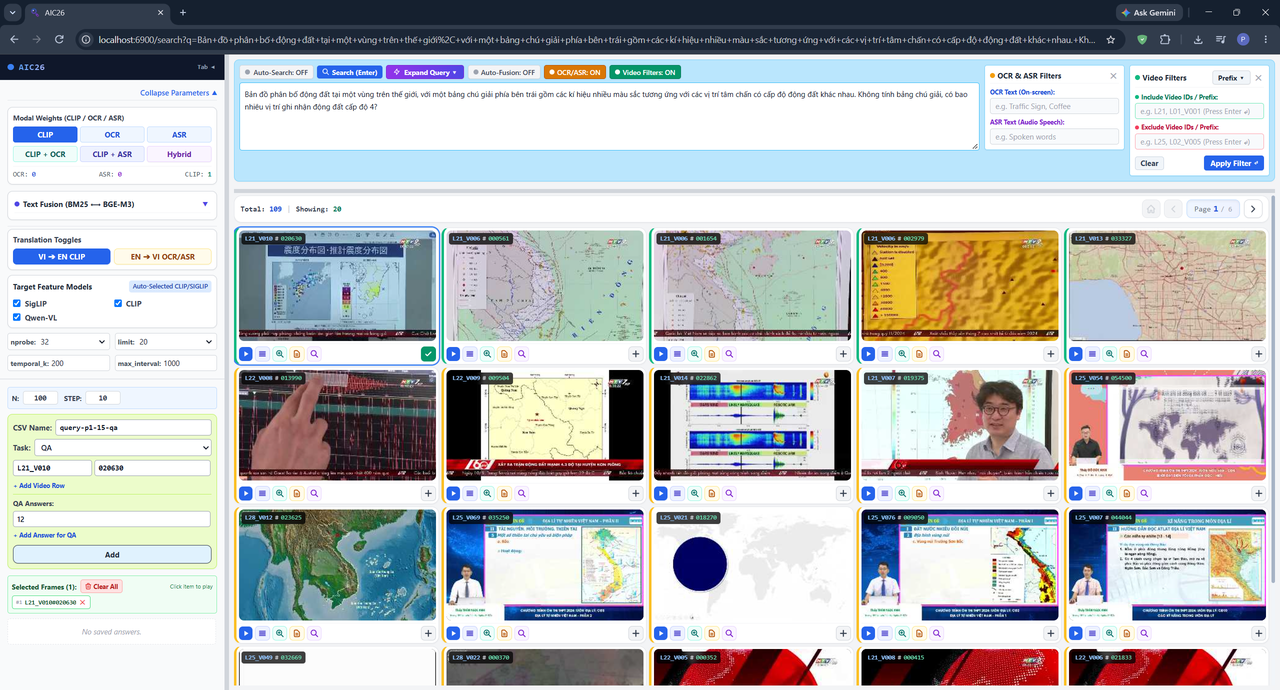
\includegraphics[width=\linewidth]{sample1.png}\\[2pt]
    {\footnotesize (a) \textbf{Query Formulation \& QA Console:} Multi-modal console supporting natural language queries, modal weight allocation (Visual/OCR/ASR), encoder selection (\texttt{SigLIP}, \texttt{OpenCLIP}, \texttt{Qwen-VL}), and left QA inspection panel (\texttt{L21\_V010\#020630}, target answer = 12) with Rank-1 ground-truth target confirmation.}
    \label{fig:ui_query}
\end{minipage}\hfill
\begin{minipage}[t]{0.488\textwidth}
    \centering
    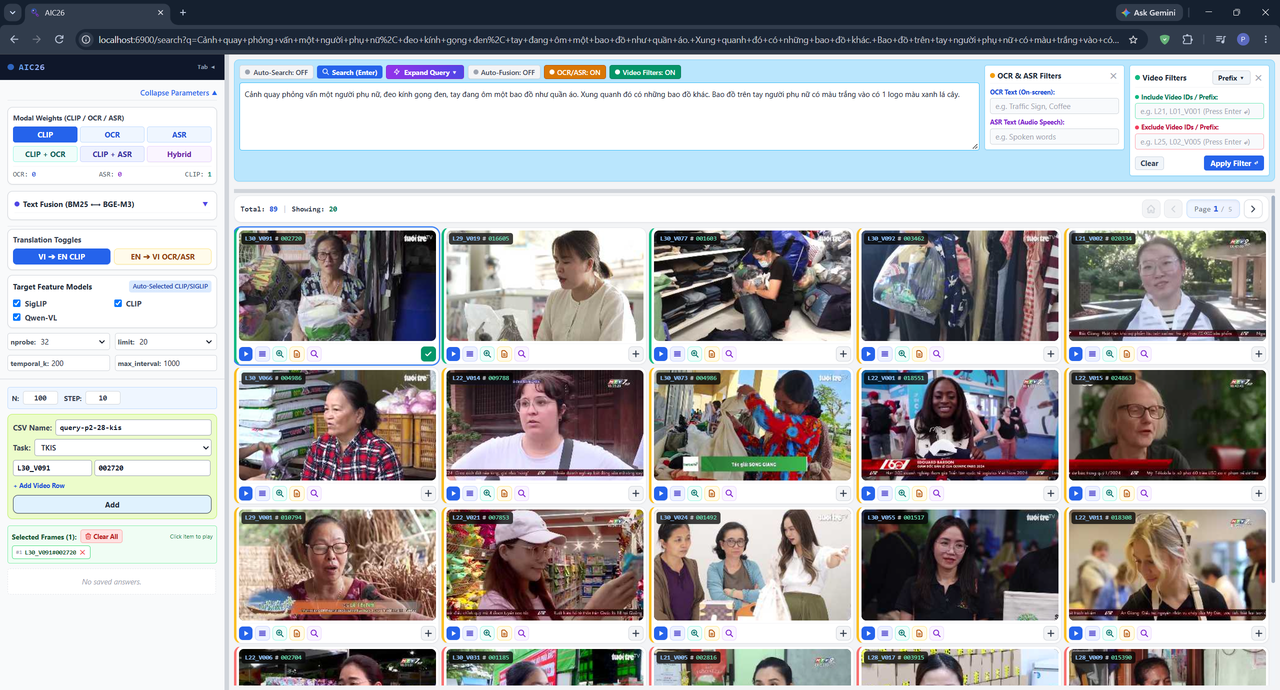
\includegraphics[width=\linewidth]{sample4.png}\\[2pt]
    {\footnotesize (b) \textbf{Diversified Result Grid:} High-density keyframe cards (20 items/page) partitioned by moving-average segment clustering to suppress visually redundant consecutive shots for a television interview query (\texttt{L30\_V091\#002720}).}
    \label{fig:ui_grid}
\end{minipage}

\vspace{0.25cm}

\begin{minipage}[t]{0.488\textwidth}
    \centering
    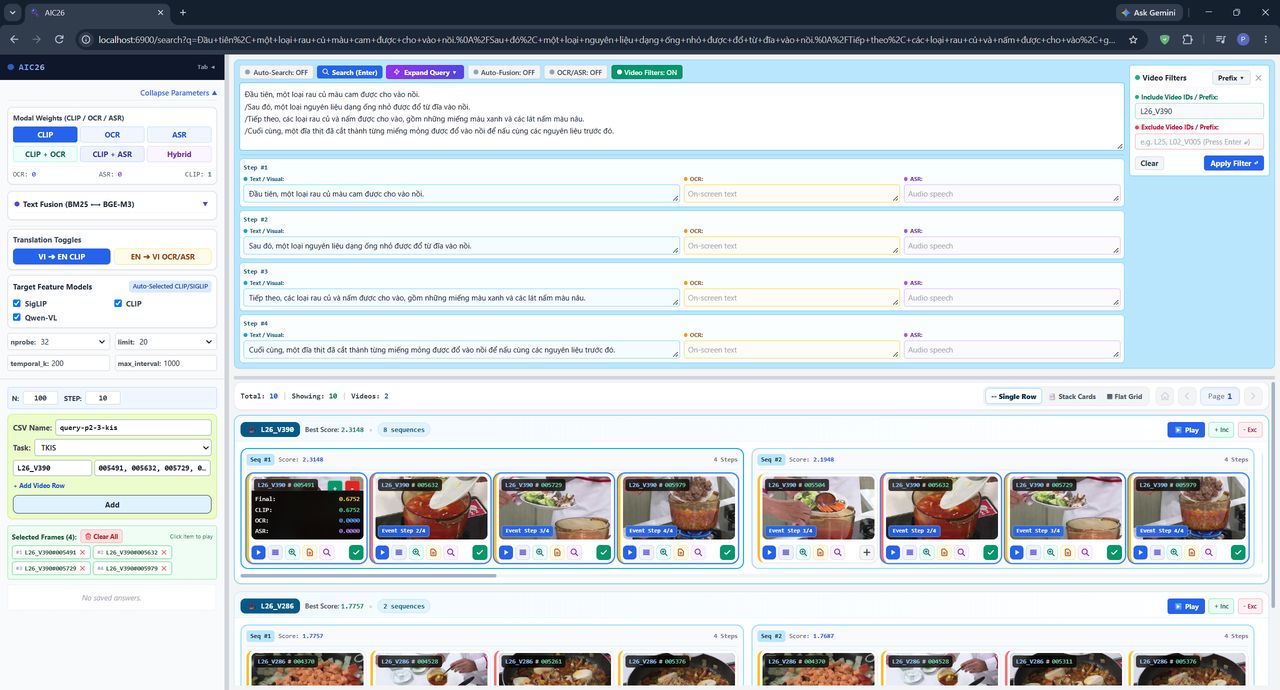
\includegraphics[width=\linewidth]{sample2.png}\\[2pt]
    {\footnotesize (c) \textbf{Temporal Sequence Alignment \& Ranking:} Grouped sequence rows (\texttt{L26\_V390}, composite score 2.3148 across 8 candidate sequences), component score breakdown (CLIP/OCR/ASR), and video prefix scoping (\texttt{L26\_V390}).}
    \label{fig:ui_filter}
\end{minipage}\hfill
\begin{minipage}[t]{0.488\textwidth}
    \centering
    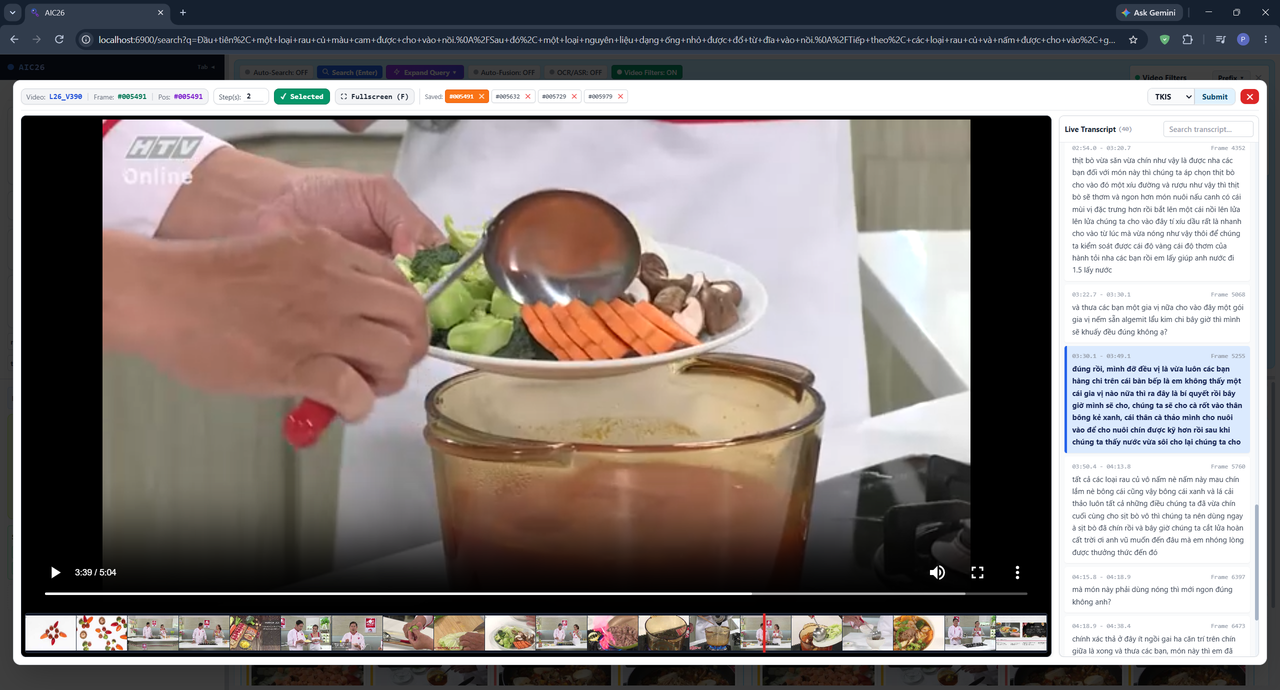
\includegraphics[width=\linewidth]{sample3.png}\\[2pt]
    {\footnotesize (d) \textbf{Precision Video Player \& Target Verification:} Modal inspection with full-width keyframe timeline strip (03:39 / 05:04), synchronized real-time WhisperX ASR transcript tracking, target selection toggles, and submission assembly.}
    \label{fig:ui_player}
\end{minipage}
\vspace{0.15cm}
\Description{The Vecna interactive retrieval workspace illustrating four core workflows: query formulation, diversified candidate browsing, temporal sequence alignment, and precision video player verification.}
\caption{The Vecna interactive retrieval workspace illustrating four core human-in-the-loop workflows: (a) Multi-modal query formulation, modality weight balancing, and QA parameter configuration; (b) Diversified result grid browsing with segment clustering; (c) Multi-step temporal sequence alignment and score decomposition; (d) High-precision video player verification with real-time speech transcript tracking and target keyframe assembly.}
\label{fig:ui_system}
\vspace{-0.25cm}
\end{figure*}

\subsection{Multi-Modal Query Formulation and QA Console (Figure~\ref{fig:ui_system}a)}
The query console serves as the entry point for expressing heterogeneous search intents. Analysts can formulate unbounded natural language descriptions or target questions. The interface exposes immediate controls to adjust modal contribution weights $w_{\text{vis}}$, $w_{\text{ocr}}$, and $w_{\text{asr}}$, dynamically tuning the convex fusion equation (\S\ref{sec:fusion}). Furthermore, operators can dynamically toggle visual representation backends (\texttt{SigLIP}, \texttt{OpenCLIP}, \texttt{Qwen-VL}) and bidirectional translation pipelines ($\text{VI} \rightarrow \text{EN}$ for visual encoders and $\text{EN} \rightarrow \text{VI}$ for OCR/ASR channels). For Question Answering (QA) tasks, the dedicated left panel enables operators to bind candidate video frames (e.g., \texttt{L21\_V010\#020630}) with textual or numeric deductions, confirming Rank-1 targets with high visual salience.

\subsection{Diversified Candidate Browsing via Segment Clustering (Figure~\ref{fig:ui_system}b)}
The candidate search view presents a high-density, paginated grid rendering 20 keyframe cards per page. Because raw video streams contain extensive temporal redundancy where consecutive frames exhibit near-identical visual representations, the grid is directly filtered through our moving-average segment clustering manifold (\S\ref{sec:diversify}). Each card corresponds to a distinct temporal segment boundary, displaying the segment badge, relative timestamp, and similarity confidence score. Each card equips the analyst with instant operational triggers: sub-frame video playback, localized OCR string inspection, image-to-image nearest-neighbor search, and direct submission staging.

\subsection{Temporal Sequence Refinement and Score Breakdown (Figure~\ref{fig:ui_system}c)}
For complex temporal activities spanning sequential phases (e.g., the culinary preparation sequence in \texttt{query-p2-3-kis}), the interface switches to a sequence-aligned grouping view. Candidates satisfying the forward temporal constraint are organized by video identifier (e.g., \texttt{L26\_V390} displaying an optimal alignment score of 2.3148 across 8 plausible step trajectories). The card visually unpacks each chronological step (Step 1/4 through Step 4/4), accompanied by decomposed similarity scores for visual semantics, optical text, and speech transcription. This transparent attribution empowers the analyst to verify step-by-step continuity and batch-select verified sequence tuples into the submission queue with a single keystroke.

\subsection{Precision Verification and Synchronized Transcript Tracking (Figure~\ref{fig:ui_system}d)}
Clicking any candidate activates the precision inspection modal, engineered for zero-latency verification:
\begin{itemize}
    \item \textbf{Synchronized Video Player:} Employs a custom HTML5 canvas-accelerated video renderer coupled to a full-width timeline strip. The timeline marks all indexed keyframes, permitting instantaneous scrubbing between global video context and localized micro-events.
    \item \textbf{Live WhisperX Transcript Scrolling:} The right-hand panel renders timestamped speech transcripts generated by WhisperX Turbo. As the video progresses, the active dialogue segment is dynamically highlighted and auto-scrolled, enabling rapid verification of verbal clues.
    \item \textbf{Sub-Frame Stepping \& Snapping:} Analysts can execute discrete frame-by-frame steps ($\pm 1/\text{FPS}$) or snap directly to adjacent keyframe boundaries without taking their hands off the keyboard.
\end{itemize}

\begin{table}[t]
\centering
\caption{Taxonomy of Zero-Latency Keyboard Interactions}
\label{tab:shortcuts}
\begin{tabular}{ll}
\toprule
\textbf{Interaction Modality} & \textbf{Keybinding} \\
\midrule
Focus Search Console & \texttt{/} \\
Instant Inspection (Candidates 1--10) & \texttt{Shift} + \texttt{1..0} \\
Sub-Frame Stepping ($\pm \frac{1}{\text{FPS}}$) & \texttt{[} / \texttt{]} or \texttt{Shift} + $\leftarrow/\rightarrow$ \\
Adjacent Keyframe Snapping & \texttt{Ctrl} + $\leftarrow/\rightarrow$ \\
Playback Modulation (Play/Pause) & \texttt{K} \\
Playback Speed ($0.25\times$--$4.0\times$) & \texttt{+} / \texttt{-} \\
Candidate Selection / Toggle & \texttt{S} \\
Batch Sequence / Payload Submission & \texttt{Shift} + \texttt{Enter} \\
\bottomrule
\end{tabular}
\end{table}

\subsection{Keyboard-Driven Navigation and Operational Ergonomics}
Biomechanical analysis in operational IR environments shows that frequent context switches between keyboard input and mouse manipulation severely degrade retrieval velocity. Vecna formalizes an ergonomic keyboard-first navigation scheme (Table~\ref{tab:shortcuts}). Core temporal primitives, modal inspection, and submission triggers are mapped to zero-latency shortcuts, allowing analysts to iterate through candidate hypotheses without tactile disruption.

\subsection{Four-Tier Operational Escalation Protocol}
To maximize recall and precision under strict session countdowns, operators adhere to a structured four-tier escalation strategy:
\begin{enumerate}[label=\textbf{Tier \arabic*:}, leftmargin=*]
    \item \textbf{Direct Zero-Shot Baseline:} Query the verbatim prompt utilizing automated translation ($\text{VI} \rightarrow \text{EN}$) and dense multi-vector embeddings (OpenCLIP, SigLIP, or Qwen3-VL).
    \item \textbf{Semantic Decomposition \& Anchor Extraction:} If direct retrieval proves ambiguous, decompose the query into core visual anchors, filtering out background clutter and non-essential grammatical tokens.
    \item \textbf{Multi-Modal Enrichment via OCR and ASR:} Activate text channels by specifying on-screen text overlays (\texttt{[ocr:...]}) or spoken keywords (\texttt{[asr:...]}), matched against BGE-M3 dense vectors and BM25 inverted indexes.
    \item \textbf{Domain Batch Priors \& Negative Video Filtering:} Restrict search scope using thematic archive heuristics (e.g., batch \texttt{L26}) and prune non-target video clusters via negative exclusion (\texttt{[!video:L26\_Vxxx]}), while dynamic replenishment continuously backfills valid candidates.
\end{enumerate}

\subsection{Adaptive Frame Expansion and Provenance Export}
When target events span ambiguous boundaries, the interface provides dynamic symmetric frame expansion. For focal frame $f^*$, radius $n$, and step magnitude $\delta$, the system deterministically populates the candidate set $\{f^* \pm k\delta\}_{k=1}^n$ within video domain $[0, F_{\max}]$. Finally, all submission payloads are exported as CSV formatted files prepended with the UTF-8 Byte Order Mark (BOM, \texttt{U+FEFF}), ensuring cross-platform character preservation for Vietnamese text during automated evaluation.

\section{Conclusion}\label{sec:conclusion}

This work introduces Vecna, a comprehensive multimedia information retrieval framework designed to systematically resolve four fundamental challenges in large-scale video search (RC1-RC4). By synthesizing factual Hypothetical Document Embeddings (HyDE) for robust query expansion, hybrid semantic-lexical fusion for robust retrieval, dynamic programming for temporal alignment, and diversification schemas for result presentation, Vecna substantially elevates retrieval efficacy. The incorporation of rigorous provenance tracking throughout the pipeline further ensures the interpretability and reliability of the retrieval outcomes in high-stakes operational environments.

Extensive empirical evaluations substantiate the superiority of the proposed framework. Vecna achieves a Recall@20 of 0.917 and a Mean Reciprocal Rank (MRR) of 0.668, representing a formidable $+34.2\%$ improvement over existing state-of-the-art baselines. Crucially, these accuracy gains are realized without compromising computational efficiency; the system maintains sub-second query latency and exhibits a $5.02\times$ acceleration in indexing throughput, thereby satisfying the rigorous performance constraints of time-critical retrieval tasks.

Despite these advancements, certain architectural limitations remain. Currently, feature embeddings are generated strictly per isolated static keyframe rather than continuous video segments, which constrains the system's capacity for fine-grained action understanding, motion dynamics, and semantic transitions between entities. Furthermore, the absence of pre-computed dense keyframe captions occasionally limits long-form narrative matching. Future work will investigate offline dense captioning via frontier vision-language models, the integration of lightweight video clip representations for end-to-end spatio-temporal reasoning, and pre-computed multi-scale keyframe crops for enhanced small-object detection. Additionally, extending the provenance tracking framework to federated verification protocols across distributed media archives presents a vital trajectory for ensuring verifiable data integrity at scale.


\bibliographystyle{splncs04}
\bibliography{references}

\end{document}
